\documentclass[tikz,border=15pt]{standalone}
\usetikzlibrary{shapes,calc,arrows,through,intersections}
\usepackage{xcolor}
\begin{document}

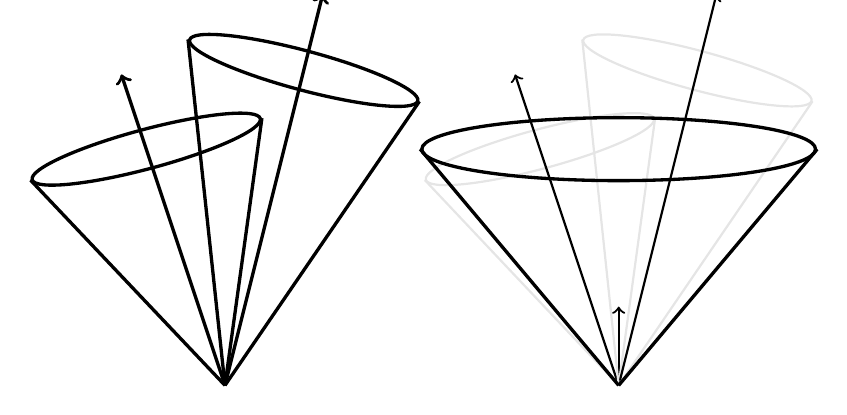
\begin{tikzpicture}

  % \draw[step=1.0,thin,gray] (-5,0) grid (14,5);
  % \begin{scope}
  %   \clip (-2,0) rectangle (2,1cm);
  %   \draw[dashed] (0,0) circle(2cm and 0.35cm);
  % \end{scope}
  \draw (-1,3) node (jet1) [very thick,rotate=15,ellipse, minimum height=0.5cm,minimum width=3cm,draw] {};
  \draw (1,4) node (jet2) [very thick,rotate=-15,ellipse, minimum height=0.5cm,minimum width=3cm,draw] {};
  % \draw[thick,->] (0,0) -- node[left,font=\footnotesize] {$x$} (0,4);
  % \draw (aa) -| (bb);
  \draw[->, very thick, shorten >=-1cm] (0,0) -- (-1,3);
  \draw[very thick] (0,0) -- (jet1.west);
  \draw[very thick] (0,0) -- (jet1.east);

  \draw[->, very thick, shorten >=-1cm] (0,0) -- (1,4);
  \draw[very thick] (0,0) -- (jet2.west);
  \draw[very thick] (0,0) -- (jet2.east);

  \begin{scope}[shift={(5,0)}]

  \draw (-1,3) node (jet1) [gray!20,thick,rotate=15,ellipse, minimum height=0.5cm,minimum width=3cm,draw] {};
  \draw (1,4) node (jet2) [gray!20,thick,rotate=-15,ellipse, minimum height=0.5cm,minimum width=3cm,draw] {};
  % \draw[thick,->] (0,0) -- node[left,font=\footnotesize] {$x$} (0,4);
  % \draw (aa) -| (bb);

  \draw[->, thick] (0,0) -- (0,1);
  \draw[->, thick, shorten >=-1cm] (0,0) -- (-1,3);
  \draw[gray!20,thick] (0,0) -- (jet1.west);
  \draw[gray!20,thick] (0,0) -- (jet1.east);

  \draw[->, thick, shorten >=-1cm] (0,0) -- (1,4);
  \draw[gray!20,thick] (0,0) -- (jet2.west);
  \draw[gray!20,thick] (0,0) -- (jet2.east);


  \draw (0,3) node (jet) [very thick,rotate=0,ellipse, minimum height=0.8cm,minimum width=5cm,draw] {};
  \draw[very thick] (0,0) -- (jet.west);
  \draw[very thick] (0,0) -- (jet.east);

  \end{scope}

\end{tikzpicture}
\end{document}
